% ===========================================================
%  Лекция 10. Задача о максимальном потоке.
%             Алгоритм Форда—Фалкерсона
% ===========================================================

\chapter{Лекция 10. Алгоритм Форда—Фалкерсона}

% -----------------------------------------------------------
% Постановка задачи
% -----------------------------------------------------------
\subsection*{Постановка задачи}

\textbf{Дано:} сеть $G(V, E)$,\quad $\sigma\colon E \to \mathbb{R}$ --- пропускная
способность рёбер.

\textbf{Найти:} один из максимальных потоков $f\colon E \to \mathbb{R}_{\geq 0}$,
т.\,е. поток наибольшей мощности $|f|$.

\medskip
\noindent
Напомним (лекция~9): поток $f$ удовлетворяет ограничению $0 \le f(e) \le \sigma(e)$
и условию балансировки во всех вершинах, кроме истока $S$ и стока $F$.

% -----------------------------------------------------------
% Остаточная сеть
% -----------------------------------------------------------
\subsection*{Остаточная сеть}

\begin{defn}{Остаточная пропускная способность}{residual-capacity}
Для ребра $e = \overline{uv}$ и текущего потока $f$ \textbf{остаточная пропускная
способность} $\tilde{\sigma}(e)$ показывает, сколько ещё можно пропустить по~$e$.
Вводится обратное (фиктивное) ребро $\operatorname{inv}(e) = \overline{vu}$, и
\[
  \tilde{\sigma}(e) + \tilde{\sigma}(\operatorname{inv}(e)) = \sigma(e).
\]
Изначально $\tilde{\sigma}(e) := \sigma(e)$, $\tilde{\sigma}(\operatorname{inv}(e)) := 0$.
\end{defn}

\begin{defn}{Остаточная сеть}{residual-network}
\textbf{Остаточная сеть} --- сеть на тех же вершинах, рёбрами которой служат все рёбра
с положительной остаточной пропускной способностью $\tilde{\sigma}(e) > 0$
(включая обратные рёбра $\operatorname{inv}(e)$).
\end{defn}

\begin{defn}{Исчерпанное (насыщенное) ребро}{saturated-edge}
\textbf{Исчерпанное ребро} --- ребро с нулевой остаточной пропускной способностью
$\tilde{\sigma}(e) = 0$ (поток по нему равен пропускной способности: $f(e) = \sigma(e)$).
\end{defn}

% -----------------------------------------------------------
% Разрезы
% -----------------------------------------------------------
\subsection*{Разрезы}

\begin{defn}{Разрез в сети}{cut}
\textbf{Разрез} в сети --- такой набор рёбер $\tilde{E} \subseteq E$, что удаление его
разрывает все пути $S \to F$, т.\,е. граф $G(V,\, E \setminus \tilde{E})$ теряет
связность между $S$ и $F$.

\medskip
\textbf{NB.} Любой мост --- разрез. Обычно рассматривают $\tilde{E}$, минимальный
по включению.
\end{defn}

\begin{defn}{Главный разрез}{main-cut}
\textbf{Главный разрез} --- разрез, при котором граф делится ровно на две части.
\end{defn}

\begin{defn}{Пропускная способность разреза}{cut-capacity}
Пропускная способность разреза $\tilde{E}$ --- сумма пропускных способностей его рёбер,
направленных из части истока в часть стока:
$\displaystyle \sigma(\tilde{E}) = \sum_{e \in \tilde{E}} \sigma(e)$.
\end{defn}

% -----------------------------------------------------------
% Алгоритм
% -----------------------------------------------------------
\subsection*{Алгоритм Форда—Фалкерсона}

\begin{algo}{Форда—Фалкерсона (поиск максимального потока)}{ford-fulkerson}
\textbf{Инициализация:}
\[
  \forall\, e \in E\colon\; f(e) := 0, \qquad
  \forall\, e \in E\colon\; \tilde{\sigma}(e) := \sigma(e).
\]

\textbf{Шаг.} Пока в остаточной сети существует путь $S \xrightarrow{\;e_1\;} \cdots
\xrightarrow{\;e_t\;} F$ (дополняющий путь):

\begin{enumerate}
  \item Находим узкое место пути ---
        $\displaystyle \delta := \min_{1 \le i \le t} \tilde{\sigma}(e_i)$,
        и увеличиваем поток вдоль всего пути:
        $\forall\, e_i\colon f(e_i) \mathrel{+}= \delta$.

  \item Перестраиваем остаточную сеть: для каждого ребра пути
        \[
          \tilde{\sigma}_{\text{new}}(e_i) = \tilde{\sigma}_{\text{old}}(e_i) - \delta,
          \qquad
          \tilde{\sigma}_{\text{new}}(\operatorname{inv}(e_i))
            = \tilde{\sigma}_{\text{old}}(\operatorname{inv}(e_i)) + \delta.
        \]
\end{enumerate}

\textbf{Выход:} когда дополняющих путей больше нет, текущий поток $f$ --- максимальный.

\medskip
\noindent\textbf{Пример.} Сеть с вершинами $S, A, B, C, D, F$ (та же, что
в лекции~9). Подпись каждого ребра --- $f/\sigma$
(поток\,/\,пропускная способность). Дополняющий путь выделен оранжевым,
рёбра с положительным потоком --- зелёным. Пути ищем поиском в ширину
(кратчайший по числу рёбер --- вариант Эдмондса--Карпа).

\begin{center}\begin{tabular}{cc}
\shortstack{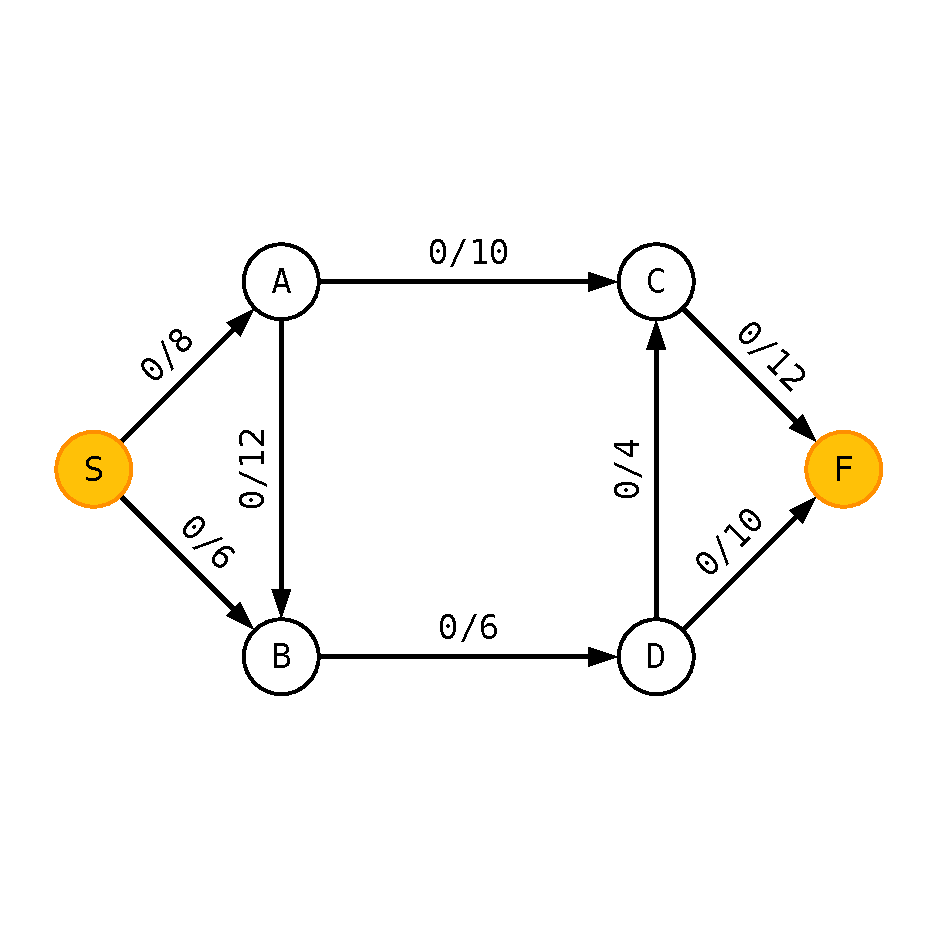
\includegraphics[width=0.46\textwidth]{python/lec10/ford_fulkerson/ford_fulkerson-0.pdf}\\[2pt]{\scriptsize Шаг 0. Инициализация: $f \equiv 0$, $\tilde\sigma = \sigma$}} &
\shortstack{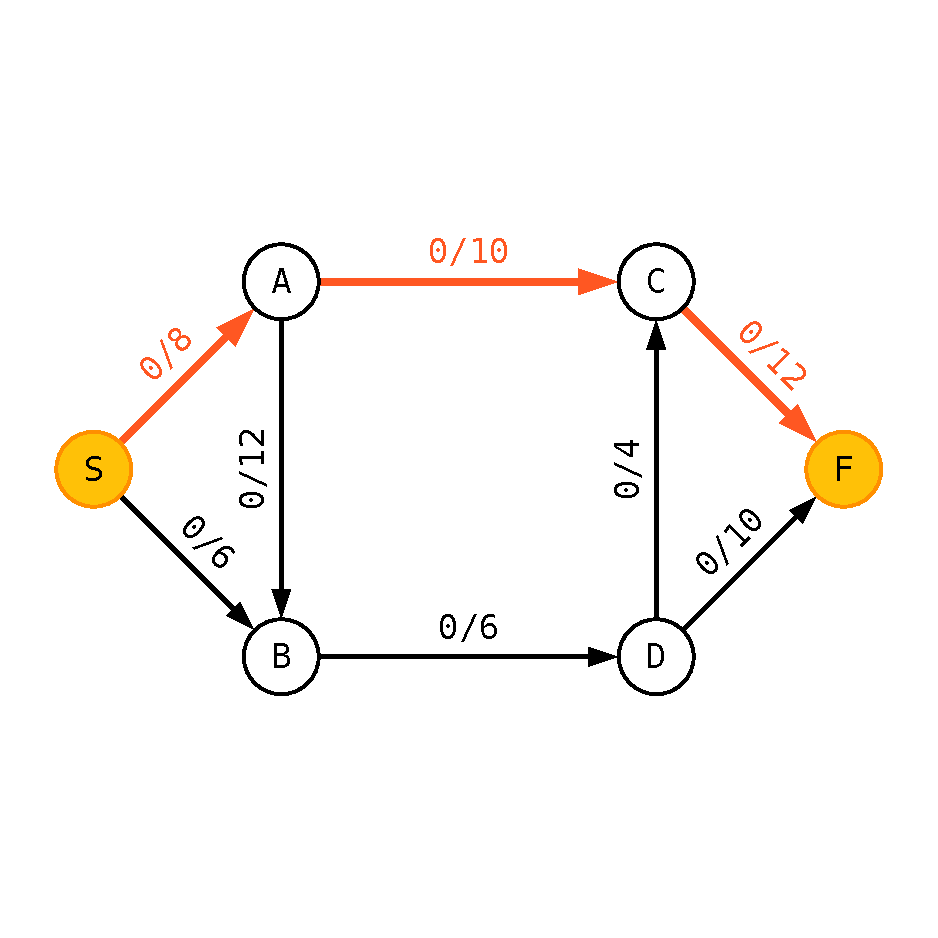
\includegraphics[width=0.46\textwidth]{python/lec10/ford_fulkerson/ford_fulkerson-1.pdf}\\[2pt]{\scriptsize Шаг 1. Путь $S{\to}A{\to}C{\to}F$, $\delta = \min(2,1,3) = 1$}} \\
\end{tabular}\end{center}
\begin{center}\begin{tabular}{cc}
\shortstack{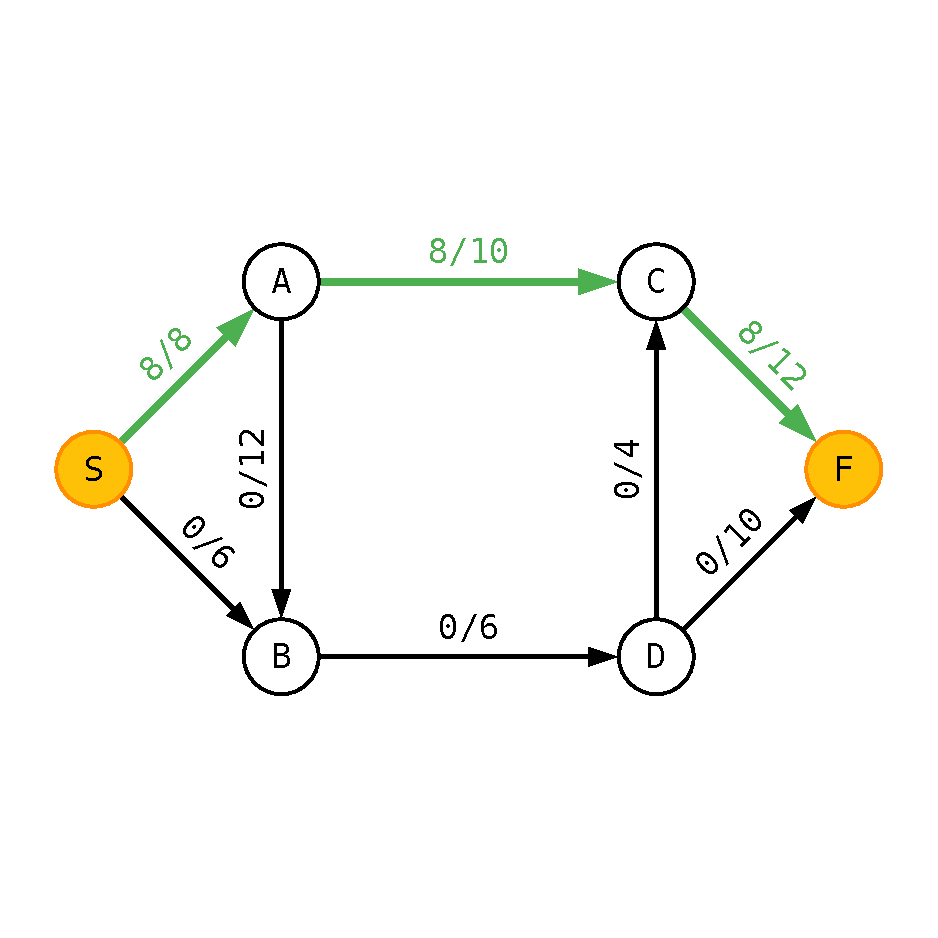
\includegraphics[width=0.46\textwidth]{python/lec10/ford_fulkerson/ford_fulkerson-2.pdf}\\[2pt]{\scriptsize Шаг 2. Поток проведён: $|f| = 1$; $A{\to}C$ исчерпано}} &
\shortstack{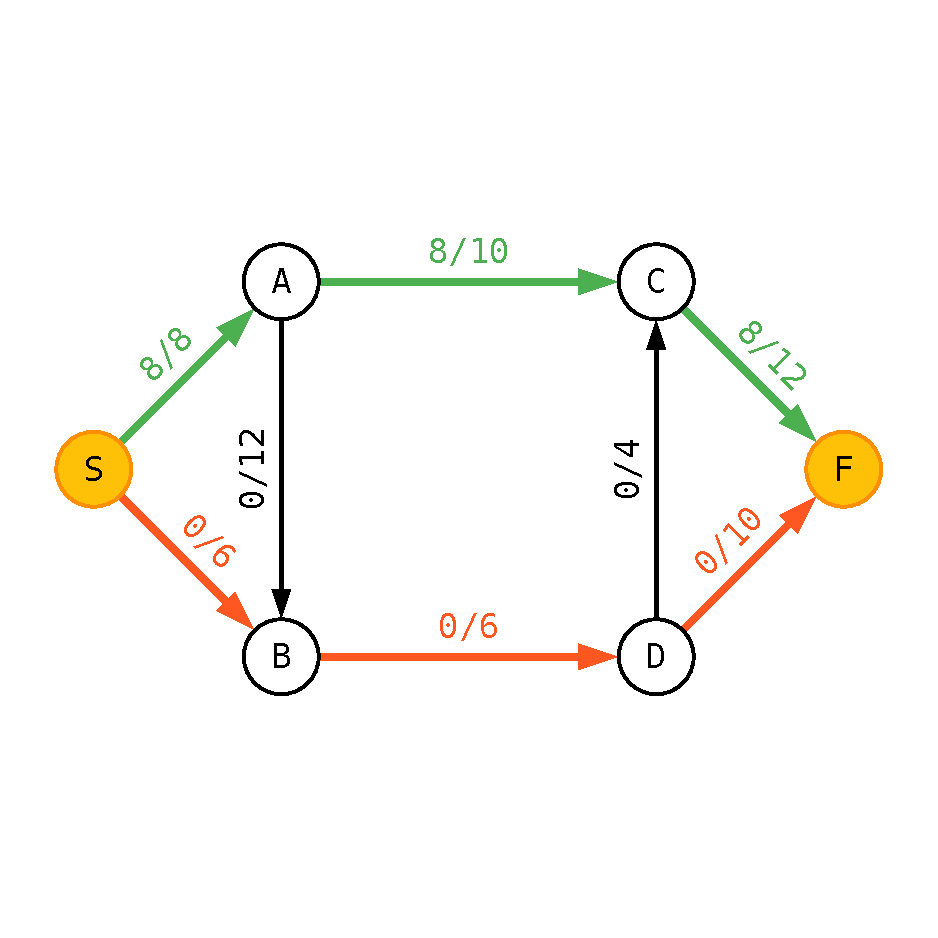
\includegraphics[width=0.46\textwidth]{python/lec10/ford_fulkerson/ford_fulkerson-3.pdf}\\[2pt]{\scriptsize Шаг 3. Путь $S{\to}B{\to}D{\to}F$, $\delta = \min(3,4,2) = 2$}} \\
\end{tabular}\end{center}
\begin{center}\begin{tabular}{cc}
\shortstack{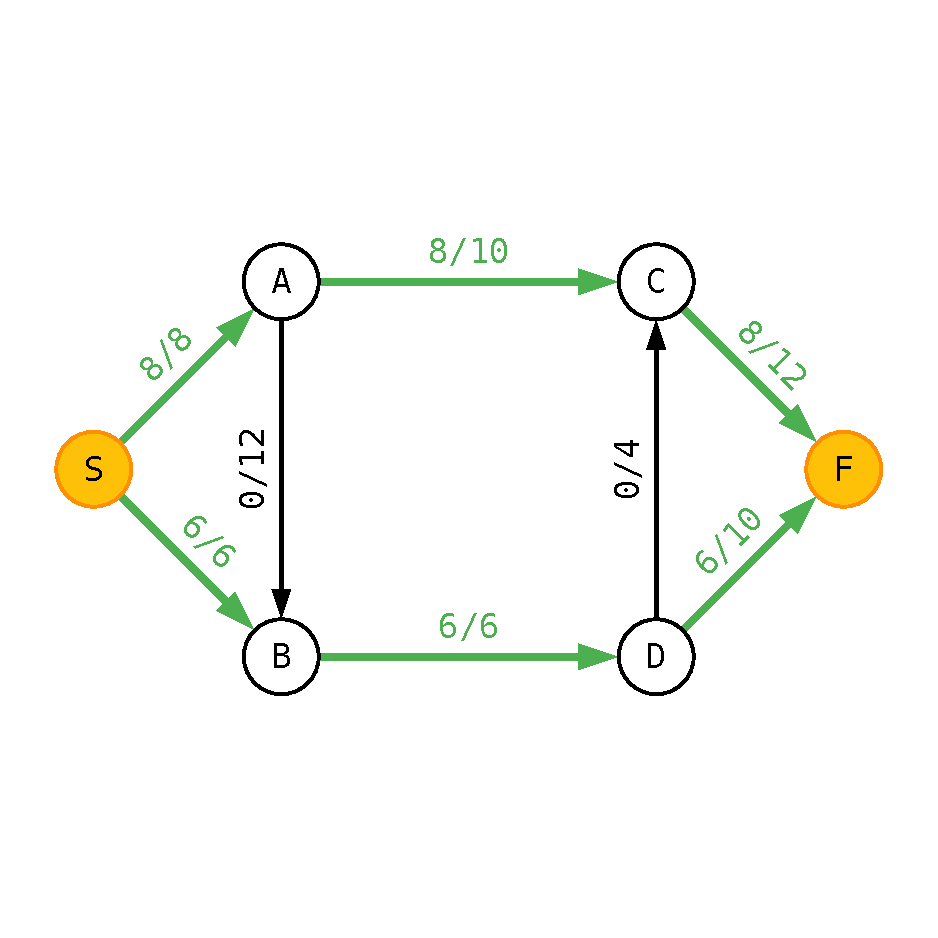
\includegraphics[width=0.46\textwidth]{python/lec10/ford_fulkerson/ford_fulkerson-4.pdf}\\[2pt]{\scriptsize Шаг 4. $|f| = 3$; ребро $D{\to}F$ исчерпано}} &
\shortstack{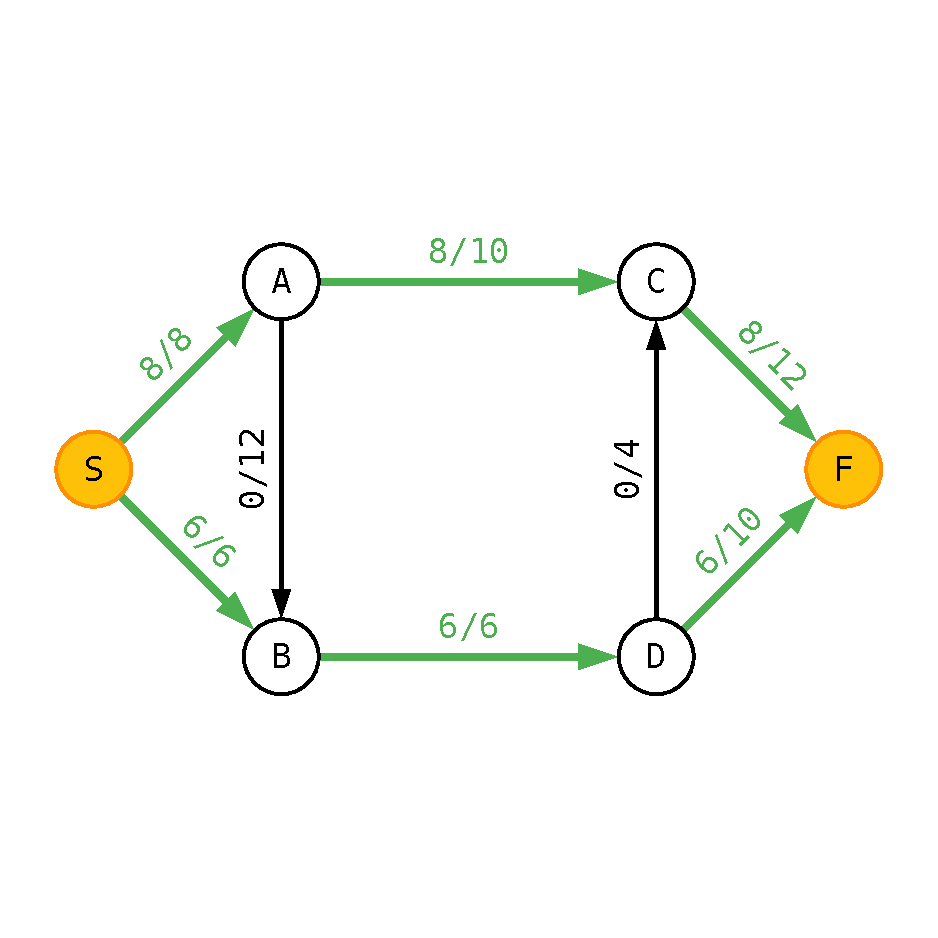
\includegraphics[width=0.46\textwidth]{python/lec10/ford_fulkerson/ford_fulkerson-5.pdf}\\[2pt]{\scriptsize Шаг 5. Путь $S{\to}B{\to}D{\to}C{\to}F$, $\delta = 1$}} \\
\end{tabular}\end{center}
\begin{center}\begin{tabular}{cc}
\shortstack{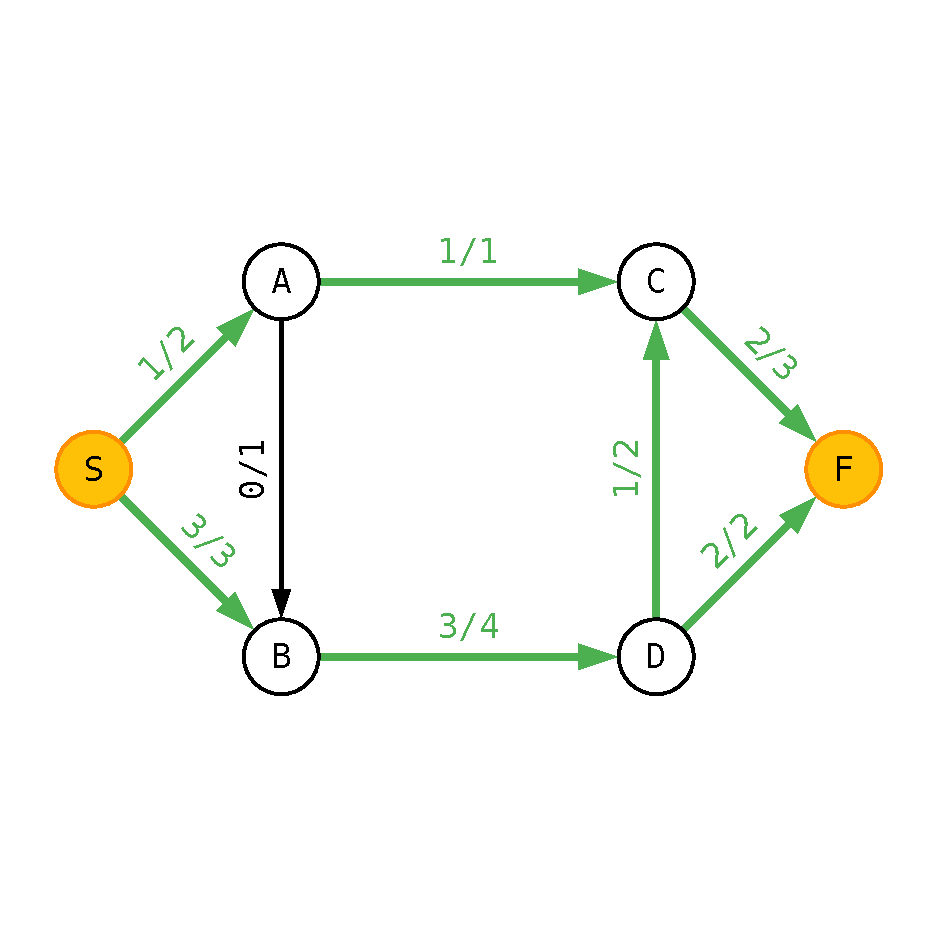
\includegraphics[width=0.46\textwidth]{python/lec10/ford_fulkerson/ford_fulkerson-6.pdf}\\[2pt]{\scriptsize Шаг 6. $|f| = 4$; ребро $S{\to}B$ исчерпано}} &
\shortstack{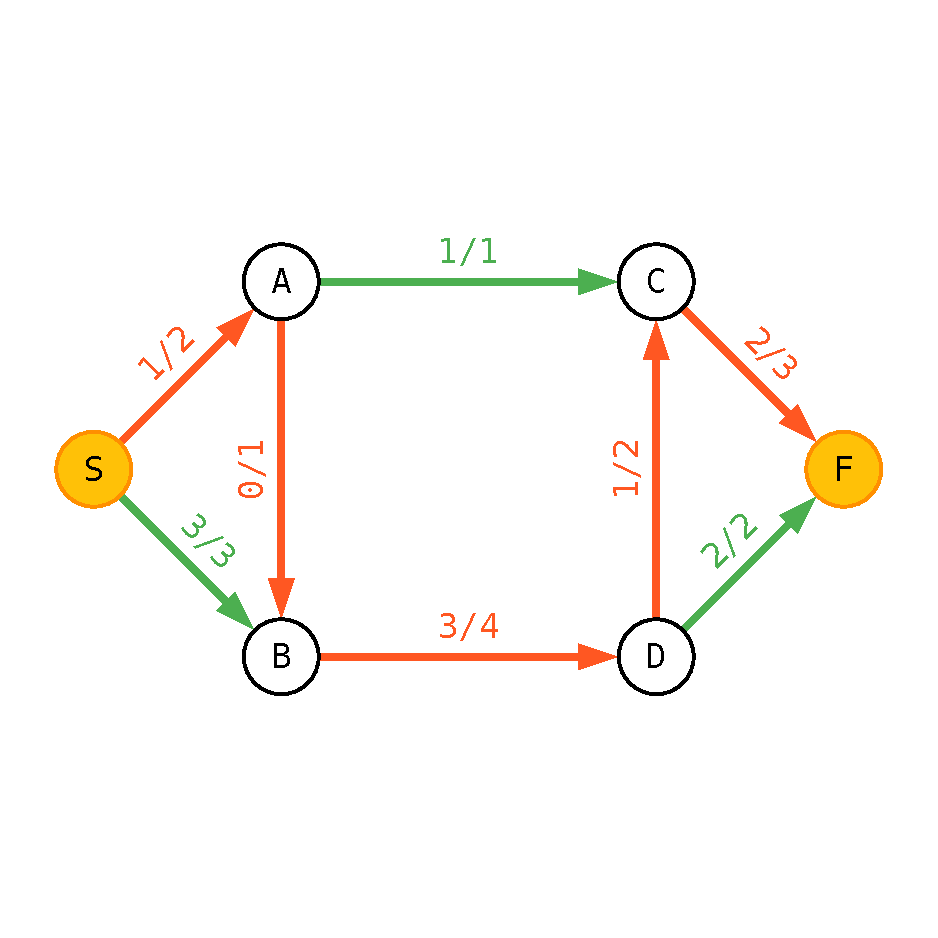
\includegraphics[width=0.46\textwidth]{python/lec10/ford_fulkerson/ford_fulkerson-7.pdf}\\[2pt]{\scriptsize Шаг 7. Путь $S{\to}A{\to}B{\to}D{\to}C{\to}F$, $\delta = 1$}} \\
\end{tabular}\end{center}
\begin{center}\begin{tabular}{cc}
\shortstack{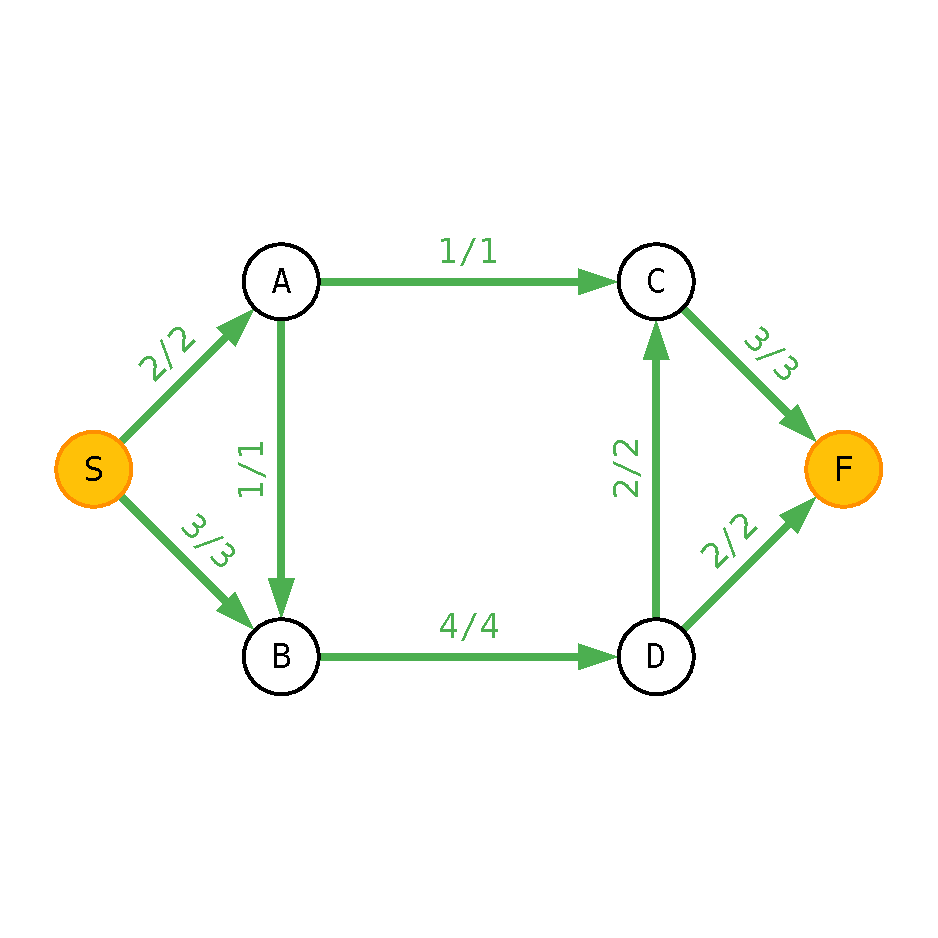
\includegraphics[width=0.46\textwidth]{python/lec10/ford_fulkerson/ford_fulkerson-8.pdf}\\[2pt]{\scriptsize Шаг 8. $|f| = 5$; ребро $S{\to}A$ исчерпано}} &
\shortstack{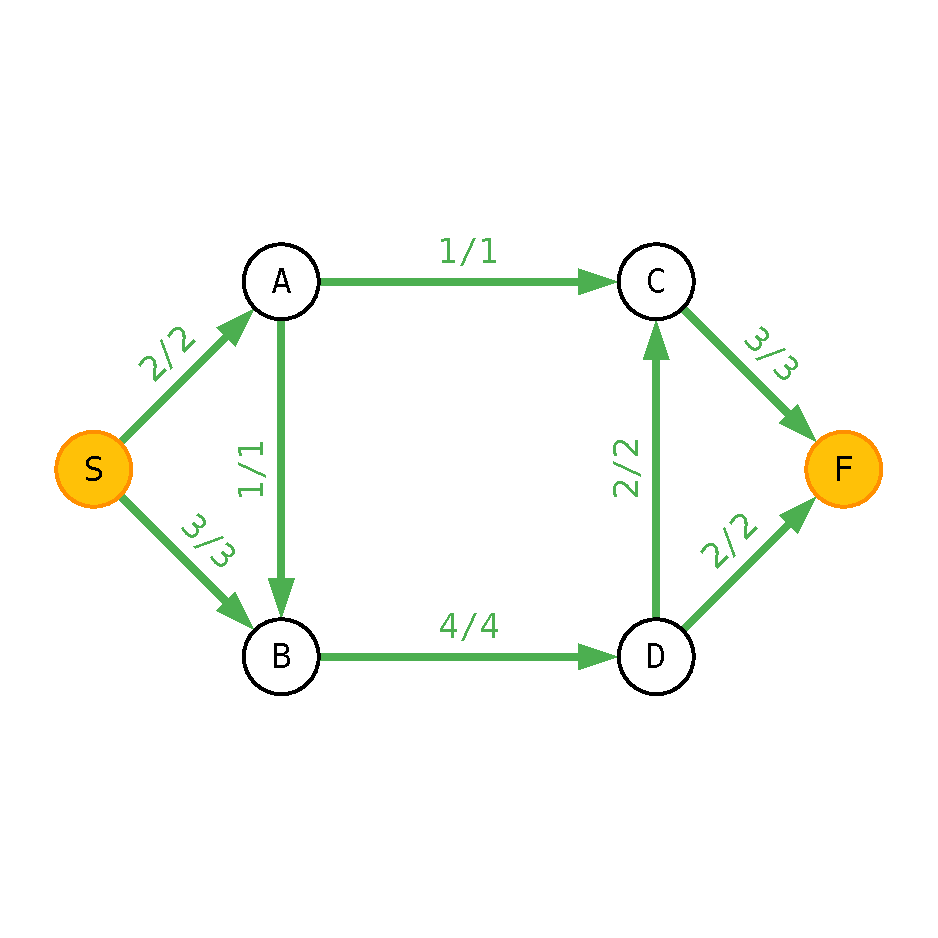
\includegraphics[width=0.46\textwidth]{python/lec10/ford_fulkerson/ford_fulkerson-9.pdf}\\[2pt]{\scriptsize Шаг 9. Путей $S \to F$ в остаточной сети нет: $|f|_{\max} = 5$}} \\
\end{tabular}\end{center}

\noindent\textit{Комментарии к шагам.} На каждом шаге величина потока
увеличивается на узкое место $\delta$ найденного пути: $1 + 2 + 1 + 1 = 5$.
После шага~8 оба ребра из истока ($S{\to}A$ и $S{\to}B$) исчерпаны:
в остаточной сети из $S$ не выходит ни одного ребра, дополняющих путей
нет --- алгоритм останавливается.

\medskip
\noindent\textbf{Проверка через разрез.} Набор рёбер
$\tilde E = \{S{\to}A,\; S{\to}B\}$ --- главный разрез
($\{S\}$ против остальных вершин) с пропускной способностью
$\sigma(\tilde E) = 2 + 3 = 5$. Мощность любого потока не превосходит
пропускной способности любого разреза, поэтому $|f| = 5 =
\sigma(\tilde E)$ --- поток максимален, а разрез минимален
(теорема Форда--Фалкерсона: $\max |f| = \min \sigma(\tilde E)$).
\end{algo}
